\documentclass{article}

\usepackage[a4paper]{geometry}

\usepackage{amssymb}
\usepackage{amsmath}
\usepackage{amsthm}
\usepackage{amsfonts}

\usepackage{multicol}

\usepackage{graphicx}
\graphicspath{ {./src} }

\usepackage{tikz}

\usepackage{pgfplots}
\pgfplotsset{compat = newest}

\usepackage{verbatim}
\usetikzlibrary{arrows,shapes}

% see https://tex.stackexchange.com/a/39755
% Simulated package file
\begin{filecontents}{envcode.sty}
      \newcommand\NewEnvCode[2]{%
            \expandafter\def\csname code@#1\endcsname{#2}%
            \expandafter\def\csname change@code@#1\endcsname{%
            \expandafter\let\expandafter\Code\csname code@#1\endcsname
            }%
      }
      
      \newcommand\MakeDefault{%
            \expandafter\let\expandafter\code@@default\csname code@\@currenvir\endcsname
      }
      
      \newcommand\RunEnvCode{%
            \let\Code=\code@@default
            \csname change@code@\@currenvir\endcsname
            \Code
      }
      
      \AtBeginDocument{\MakeDefault}
\end{filecontents}

\usepackage{envcode}

% for cross reference
% \usepackage{hyperref}

% for fixed length of cell of tables
% \usepackage{tabularx}
% \usepackage{longtable}

\newtheorem{definition}{Definition}[section]
\newtheorem{lemma}{Lemma}[section]
\newtheorem{theorem}{Theorem}[section]
\newtheorem{corollary}{Corollary}[section]
\newtheorem{proposition}{Proposition}[section]

\NewEnvCode{document}{default code}
\NewEnvCode{theorem}{ theorem }
\NewEnvCode{lemma}{ lemma }
\NewEnvCode{corollary}{ corollary }
\NewEnvCode{proposition}{ proposition }
\NewEnvCode{definition}{ definition }

\title{Communicate Without Errors}
\author{Zifan Hua}

\begin{document}
      \maketitle

      \begin{definition}[graph] \label{def:graph}
            A graph $ G $ is a set of vertices with a set of edges connecting pairs of vertices.
            \tikzstyle{vertex}=[circle,fill=black!25,minimum size=20pt,inner sep=0pt]
            \tikzstyle{edge} = [draw,thick,-]
            \tikzstyle{weight} = [font=\small]
            \begin{figure}[h!]
                  \begin{tikzpicture}[scale=1, auto,swap]
                        % Draw a 7,11 network
                        % First we draw the vertices
                        \foreach \pos/\name in {{(0,2)/a}, {(2,1)/b}, {(4,1)/c},
                              {(0,0)/d}, {(3,0)/e}, {(2,-1)/f}, {(4,-1)/g}}
                              \node[vertex] (\name) at \pos {$\name$};
                        % Connect vertices with edges and draw weights
                        \foreach \source/ \dest in {b/a, c/b,d/a,d/b,
                              e/b, e/c,e/d,
                              f/d,f/e,
                              g/e,g/f}
                            \path[edge] (\source) -- node[weight]{} (\dest);
                    \end{tikzpicture}
                    \label{fig:graphDefinitionExample}
                    \caption{An example of a graph.}
            \end{figure}
      \end{definition}

      \begin{definition}[$ \alpha(G) $] \label{def:alphaG}
            Given a graph $ G $. Given a subgraph of $ G $, $ H $, such that every vertex of $ H $ is not connected in $ G $. Then $ \alpha(G) $ is the maximum number of vertices of $ H $.
            \tikzstyle{vertex}=[circle,fill=black!25,minimum size=20pt,inner sep=0pt]
            \tikzstyle{selected vertex}=[circle,fill=red!25,minimum size=20pt,inner sep=0pt]
            \tikzstyle{edge} = [draw,thick,-]
            \tikzstyle{weight} = [font=\small]
            \begin{figure}[h!]
                  \begin{tikzpicture}[scale=1, auto,swap]
                        % Draw a 7,11 network
                        % First we draw the vertices
                        \foreach \pos/\name in {{(0,2)/a}, {(2,1)/b}, {(4,1)/c},
                              {(0,0)/d}, {(3,0)/e}, {(2,-1)/f}, {(4,-1)/g}}
                              \node[vertex] (\name) at \pos {$\name$};
                        \foreach \pos/\name in {{(0,2)/a}, {(4,1)/c},
                              {(2,-1)/f}}
                              \node[selected vertex] (\name) at \pos {$\name$};
                        % Connect vertices with edges and draw weights
                        \foreach \source/ \dest in {b/a, c/b,d/a,d/b,
                              e/b, e/c,e/d,
                              f/d,f/e,
                              g/e,g/f}
                            \path[edge] (\source) -- node[weight]{} (\dest);
                    \end{tikzpicture}
                    \label{fig:alphaGExample}
                    \caption{Example of $ \alpha(G) $. Here $ \alpha(G) = 3 $.}
            \end{figure}
      \end{definition}

      \begin{definition}[graph product]\label{def:graphProduct}
            Given two graph $ G $ and $ H $. The graph product $ G \times H $ is the graph with vertices $ V(G \times H) = V(G) \times V(H) $ in which $ (x,y) $ is adjacent to $ (x',y') $ in $ G \times H $ if and only if $ x $ is adjacent to $ x' $ in $ G $ and $ y $ is adjacent to $ y' $ in $ H $.

            A graph $ G $ product itself for $ n $ times will always be denoted by $ G^n $.
      \end{definition}

      \begin{lemma}\label{lemma:alphaIncreasing}
            Given graph $ G $ and $ H $.
            \begin{equation}
                  \alpha(G \times H) \geq \alpha(G) \alpha(H)
            \end{equation}
      \end{lemma}

      \begin{proof}
            Given graph $ G $ and $ H $. Let $ G' $ and $ H' $ be subgraph of $ G $ and $ H $ such that no vertex of $ G' $ or $ H' $ is adjacent in $ G $ or $ H $, respectively. Then $ G' \times H' $ is a subgraph of $ G \times H $ such that no vertex of $ G' \times H' $ is adjacent in $ G \times H $.
      \end{proof}

      \begin{definition}[Shannon capacity]\label{def:shannonCapacity}
            Given a graph $ G $, the Shannon capacity $ \Theta(G) $ is defined by
            \begin{equation}
                  \Theta(G) = \lim_{n \to \infty} \sqrt[n]{\alpha(G^n)} 
            \end{equation}

            We will see that this sequence is monotonically increasing and has an upper bound later. So, this sequence will always converge.
      \end{definition}

      \begin{definition}[adjacency matrix]\label{def:adjacencyMatrix}
            Given a graph $ G $, the adjacency matrix $ A $ is defined by
            \begin{equation}
                  A_{ij} = \begin{cases}
                        1 & \text{if $ i $ and $ j $ are adjacent in $ G $} \\
                        0 & \text{otherwise}
                  \end{cases}
            \end{equation}
      \end{definition}

      \begin{definition}[orthonormal representation]\label{def:orthonormalRepresentation}
            Given a graph $ G $ with vertices $ 1,2,\dots,n $, the orthonormal representation of $ G $ is a set of unit vectors $ \{v_1, v_2, \dots, v_n\} $ such that if $ i $ and $ j $ are not adjacent in $ G $, then $ v_i $ and $ v_j $ are orthogonal.
      \end{definition}

      \begin{lemma}[existence of orthonormal representation]\label{lemma:existenceOfOrthonormalRepresentation}
            Given a graph $ G $ with vertices $ 1,2,\dots,n $, there exists an orthonormal representation of $ G $.
      \end{lemma}

      \begin{proof}
            Any orthonormal basis of $ \mathbb{R}^n $ can be used as an orthonormal representation of $ G $.
      \end{proof}

      \begin{definition}[tensor product]\label{def:tensorProduct}
            Given two vectors $ v = \left(v_{1},\dots,v_{n}\right) $ and $ w = \left(w_{1},\dots,w_{n}\right) $, the tensor product $ v \circ w $ is defined by
            \begin{equation}
                  v \circ w = \left(
                        v_{1}w_{1},\dots,v_{1}w_{n},
                        v_{2}w_{1},\dots,v_{2}w_{n},
                        \dots,
                        v_{n}w_{1},\dots,v_{n}w_{n}
                        \right)
            \end{equation}
      \end{definition}

      \begin{lemma}[inner product of tensor product]\label{lemma:innerProductOfTensorProduct}
            Given two vectors $ v = \left(v_{1},\dots,v_{n}\right) $ and $ w = \left(w_{1},\dots,w_{n}\right) $, the inner product of $ v \circ w $ is defined by
            \begin{equation}
                  \langle v \circ w, v' \circ w' \rangle = \langle v, v' \rangle \langle w, w' \rangle
            \end{equation}
            
      \end{lemma}

      \begin{lemma}[product of orthonormal representation]\label{lemma:productOfOrthonormalRepresentation}
            Given a graph $ G $ with vertices $ 1,2,\dots,n $, and a graph $ H $ with vertices $ 1,2,\dots,m $. Then vectors $\{ v_{i}\circ w_{j} \}$ is an orthonormal representation of $ G \times H $.
      \end{lemma}

      \begin{definition}[value of a orthonormal representation]\label{def:valueOfOrthonormalRepresentation}
            Given an orthonormal representation $ \{v_1, v_2, \dots, v_n\} $ of a graph $ G $ the value of the representation is defined by
            \begin{equation}
                  \text{value}(\{v_1, v_2, \dots, v_n\}) = \inf_{c}\max_{i} \frac{1}{\left<c,v_{i}\right>^2}
            \end{equation}
            which $ i=1,2,\dots,n $ and c is any vector does not orthogonal to $ v_i $.
      \end{definition}

      \begin{definition}[$ \theta(G) $]\label{def:thetaFunction}
            Given a graph $ G $, the $ \theta(G) $ is defined by
            \begin{equation}
                  \theta(G) = \inf_{\{v_1, v_2, \dots, v_n\}} \text{value}(\{v_1, v_2, \dots, v_n\})
            \end{equation}
            where $ \{v_1, v_2, \dots, v_n\} $ is an orthonormal representation of $ G $.
      \end{definition}

      \begin{lemma}
            Given graph $ G $ and $ H $, then
            \begin{equation}
                  \theta(G \times H) \leq \theta(G) \theta(H)
            \end{equation}
      \end{lemma}

      \begin{proof}
            Let $ \{v_1, v_2, \dots, v_n\} $ and $ \{w_1, w_2, \dots, w_m\} $ be orthonormal representation of $ G $ and $ H $and $ c_{v} $ and $ c_{w} $ such that
            \begin{equation}
                  \max \left\{ \frac{1}{\left<c_{v},v_{i}\right>^2} : i=1,2,\dots,n \right\} = \theta(G)
            \end{equation} 
            and 
            \begin{equation}
                  \max \left\{ \frac{1}{\left<c_{w},w_{i}\right>^2} : i=1,2,\dots,m \right\} = \theta(H)
            \end{equation}

            Then
            \begin{eqnarray}
                  \theta(G \times H) &\leq& 
                  \max \left\{ \frac{1}{\left<c_{v} \circ c_{w},v_{i} \circ w_{j}\right>^2} \right\} \\
                  &=& \max \left\{ \frac{1}{\left<c_{v},v_{i}\right>^2 \left<c_{w},w_{j}\right>^2} \right\} \\
                  &=& \max \left\{ \frac{1}{\left<c_{v},v_{i}\right>^2} \right\} \max \left\{ \frac{1}{\left<c_{w},w_{j}\right>^2} \right\} \\
                  &=& \theta(G) \theta(H) \\
            \end{eqnarray}
      \end{proof}

      \begin{lemma}
            \begin{equation}
                  \theta(G) \geq \alpha(G)
            \end{equation}
      \end{lemma}

      \begin{proof}
            Let $ \{1,2,\dots,k\} $ be the set of vertices of $ G $ such that every point is not adjacency in $ G $. And $ k = \alpha(G) $

            Let $ \{v_1, v_2, \dots, v_n\} $ be an orthonormal representation of $ G $ and $ c $ such that
            \begin{equation}
                  \max \left\{ \frac{1}{\left<c,v_{i}\right>^2} \right\} = \theta(G)
            \end{equation}
                  
            Then
            \begin{eqnarray}
                  1 &=& c^{2} \\
                  &\geq& \sum_{i=1}^{k} \left<c,v_{i}\right>^{2} \\
                  &\geq& \frac{k}{\theta(G)}
            \end{eqnarray}
      \end{proof}

      \begin{theorem}
            Given a graph $ G $, then
            \begin{equation}
                  \theta(G) \geq \Theta(G)
            \end{equation}
      \end{theorem}

      \begin{proof}
            \begin{eqnarray}
                  \Theta(G) &=& \lim_{n} \sqrt[n]{\alpha(G^{n})} \\
                  &\leq& \lim_{n} \sqrt[n]{\theta(G^{n})} \\
                  &\leq& \lim_{n} \sqrt[n]{\theta(G)^{n}} \\
                  &=& \theta(G)
            \end{eqnarray}
      \end{proof}

      \begin{theorem}
            For odd $ n $,
            \begin{equation}
                  \theta(C_{n}) \geq \frac{n\cos(\pi/n)}{
                        \cos(\pi/n)+1
                  }
            \end{equation} 
      \end{theorem}

      \begin{proof}
            Consider an umbrella that has a handle and $n$ ribs that all have unit length.

            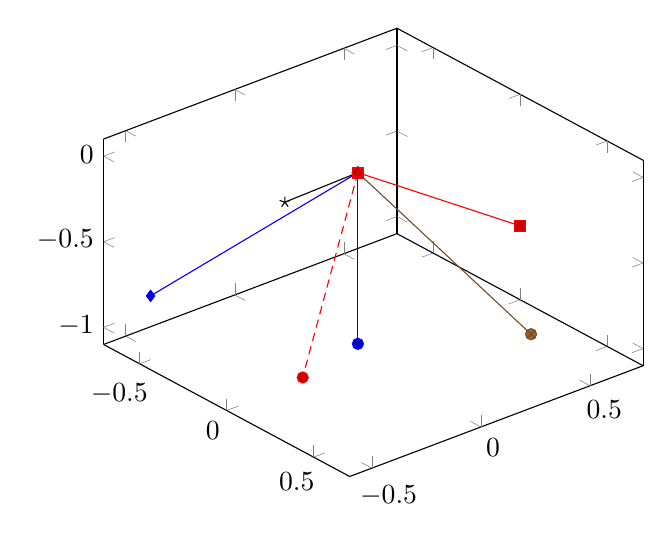
\begin{tikzpicture}
 
                  \begin{axis}[view = {50}{40}]
                   
                  \addplot3 coordinates 
                  {
                      (0,0,0)
                      (0,0,-1)
                  };

                  \addplot3 coordinates 
                  {
                      (0,0,0)
                      (0,0.74349606,-0.66874031)
                  };
                   
                  \addplot3 coordinates 
                  {
                      (0,0,0)
                      (0.70710677,0.22975292,-0.66874031)
                  };

                  \addplot3 coordinates 
                  {
                      (0,0,0)
                      (-0.70710677,0.22975292,-0.66874031)
                  };


                  \addplot3 coordinates 
                  {
                      (0,0,0)
                      (-0.43701602,-0.60150095,-0.66874031)
                  };
                  
                  \addplot3 coordinates 
                  {
                      (0,0,0)
                      (0.43701602,-0.60150095,-0.66874031)
                  };

                  \end{axis}
                   
            \end{tikzpicture}
      
            Hear, angles between two consecutive ribs are same. Let $v$ be a rib. And let $w$ be one of the rib that have the largest angle with $v$. Then, we let the angle between $v$ and $w$ be $ \pi/2 $.

            Then, the $n$ ribs of such an umbrella form an orthonormal representation of $\bar{C_{n}}$.

            Let $d$ be the vector represent the handle, and $v_{1},v_{2},\dots,v_{n}$ be the $n$ ribs. And let $\gamma$ be the angle between the handle and any rib.

            So, by some calculation, we get
            \begin{eqnarray}
                  \theta(C_{n}) &=& \max \sum_{i=1}^{n}(d^{T}v_{i})^{2} \\
                  &\ge& n\left(
                        \cos(\gamma)
                  \right)^{2} \\
                  &=& n\left(
                        \sqrt{
                              1-\frac{1}{1+\cos(\pi/n)}
                        }
                  \right)^{2} \\
                  &=& \frac{n\cos(\pi/n)}{
                        \cos(\pi/n)+1
                  }
            \end{eqnarray}
      \end{proof}

\end{document}